\documentclass[12pt]{article}
\bibliographystyle{unsrt}
\usepackage{a4wide}
\usepackage{import} 
\usepackage[utf8]{inputenc}
\usepackage[T2A]{fontenc}
\usepackage{graphics,graphicx}
\usepackage{subfig}
%\usepackage{amssymb,amsfonts,amsthm,amsmath,mathtext,cite,enumerate,float}
\usepackage{amssymb,amsfonts,amsmath,cite,enumerate,float}
\usepackage[english,russian]{babel}
\usepackage{tikz}
\usepackage{mathrsfs}
%\usepackage[noend]{algpseudocode}
%\graphicspath{home/anastasia/Anastasia/8 semestre/Воронцов/Makarova2015Thesis/Pics/} %путь к рисункам
\textheight=24cm % высота текста
\textwidth=16cm % ширина текста
\oddsidemargin=0pt % отступ от левого края
\topmargin=-1.5cm % отступ от верхнего края
\parindent=24pt % абзацный отступ
\parskip=0pt % интервал между абзацами
\tolerance=2000 % терпимость к "жидким" строкам
\flushbottom % выравнивание высоты страниц
%\graphicspath{{data/}}
\renewcommand{\baselinestretch}{1}
\renewcommand{\omega}{w}
\bibliographystyle{unsrt}
%\usepackage{mathrsfs}
%\DeclareMathOperator*{\argmin}{arg\,min}
%\usepackage{algorithm}
%\makeatlette
%\def\BState{\State\hskip-\ALG@thistlm}
%\makeatother
\renewcommand{\phi}{\varphi}
\usepackage[ruled,section]{algorithm}
\usepackage[noend]{algorithmic}

\newcommand{\argmax}{\arg\!\max}

\def\algorithmicrequire{\textbf{\textcolor{blue}{Вход:}}}
\def\algorithmicensure{\textbf{\textcolor{blue}{Выход:}}}
\def\algorithmicif{\textbf{\textcolor{blue}{если}}}
\def\algorithmicthen{\textbf{\textcolor{blue}{тогда}}}
\def\algorithmicelse{\textbf{\textcolor{blue}{иначе}}}
\def\algorithmicelsif{\textbf{\textcolor{blue}{иначе если}}}
\def\algorithmicfor{\textbf{\textcolor{blue}{для}}}
\def\algorithmicforall{\textbf{\textcolor{blue}{для всех}}}
\def\algorithmicdo{}
\def\algorithmicwhile{\textbf{\textcolor{blue}{пока}}}
\def\algorithmicrepeat{\textbf{\textcolor{blue}{повторять}}}
\def\algorithmicuntil{\textbf{\textcolor{blue}{пока}}}
\def\algorithmicloop{\textbf{\textcolor{blue}{цикл}}}

\textheight=24cm % высота текста
\textwidth=16cm % ширина текста
\oddsidemargin=0pt % отступ от левого края
\topmargin=-1.5cm % отступ от верхнего края
\parindent=24pt % абзацный отступ
\parskip=0pt % интервал между абзацами
\tolerance=2000 % терпимость к "жидким" строкам
\flushbottom % выравнивание высоты страниц


\begin{document}
\title{Makarova Anastasia}

\section{Problem1}

\subsection{1a}
Let's consider two elements a and b, then the decision boundary for element x would be equivalent to:

$$||a -x||^2 = ||b -x||^2$$
$$a^2 - 2(a,x) = b^2 - 2(b,x)$$

which corresponds to linear decision boundary.

\subsection{1b}

Let's consider a class A, then for the element x the decision rule of belonging x to A would be:

\begin{equation*}
\begin{aligned}
& \exists a \in A \ \  \forall b \notin A \\ 	
& ||a -x||^2 \leq ||b -x||^2 \\
& a^2 - 2(a,x) \leq b^2 - 2(b,x)
\end{aligned}
\end{equation*}

It would be the same for other $N - 1$ classes. So, we will receive intersection of piecewise linear curves.

\section{Problem2}

\subsection{2a}
%\input{introduction}

\begin{equation*}
cost(\hat{\omega_k}, \omega_i) = 
 \begin{cases}
   0 &\ k = i\\
   \lambda_i &\ else
 \end{cases}
\end{equation*}

\begin{itemize}
	\item Expected loss of prediction $\hat{\omega_i}$ 
	$$L(\hat{\omega_i}) = \sum_{j \ne i}^C \lambda_j p(\omega_j|x) = \sum_{j \ne i}^C \lambda_j \frac {p(\omega_j)p(x|\omega_j)}{p(x)}$$ 
	
	\item Bayes dicision rule minimizes expected loss
	$$\hat{\omega*} = \underset{\hat{\omega}}{\text{argmin}} L(\hat{\omega})$$
\end{itemize}

\subsection{2b}

$$L(\omega_i) = \sum_{j \ne i} \lambda p(\omega_j|x) = \lambda  \sum_{j \ne i} p(\omega_j|x) = \lambda ( 1 - p(\omega_i|x))$$
$$\hat{\omega*} = \underset{\hat{\omega}}{\text{argmin}} L(\hat{\omega})$$
 $$\hat{\omega*} = \underset{\hat{\omega}}{\text{argmax}} p(\hat{\omega}|x)$$
 
\section{Problem3}

\subsection{3a}
Let's consider node t, $N_t$ - number of elements at node $t$.\\
For one feature and one node t: we should do 
* $N_t$ operations with fixed threshold element to calculate probabilities of classes within the node t;\\
* do it $N_t$ times.\\
For $D$ features we have $DN_t^2$. Then let's calculate it for all nodes in the tree. If we unify nodes by levels, at each level
$$\sum_{t\in level} N_t = N$$. Then $$D\sum_{t \in level} N_t^2 \leq D\sum_{t\in level} NN_t = DN^2$$. The number of levels is equal to $log_2N$, so the result $O(DN^2logN)$  

\subsection{3b}
Let's sort features values among sample $N_t$. The cost is equal to $DNlogN$. Then the probabilities of classes within the node t will be calculated in $O(1)$, because we have a fully sorted array. Then, calculating the sum for all levels will be the same as in previous subproblem, so we have $O(DNlog^2N)$

\begin{newpage}

\section{Problem4}

\subsection{4a}
The example of misclassification can be found in a picture. Using binary tree we will have stairs as a result of making decision at each node, when a linear separability is right. 

\begin{figure}[!h]
	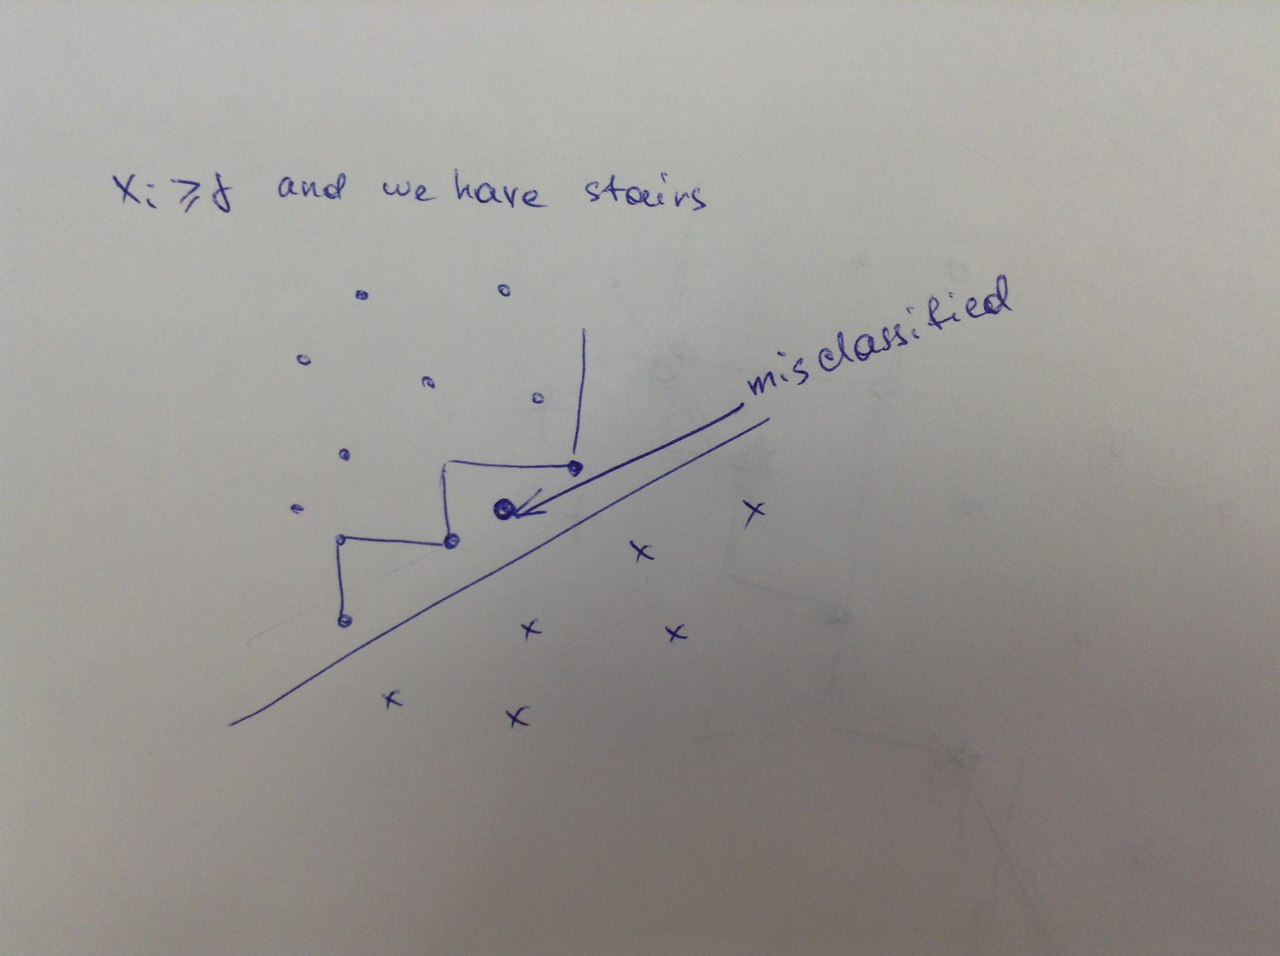
\includegraphics[width=0.6\linewidth]{ex.png}
  \caption{example of misclassification}
  \label{ExECG}
\end{figure}

\end{document}